\subsection{Deep Learning Algorithms}
\label{SubsectionDL}
Deep learning is a long established group of machine learning algorithms which has proved competence in many areas \cite{lecun2015deep}
and which have encouraged the introduction of deep learning algorithms for time series classification \cite{wang2017time}.
Deep learning is appealing for investigating time series data; due to the role that the time dimension play as a structure for the data
and because deep learning algorithms can scale linearly with training size \cite{shifaz2020ts}.

The general framework of deep learning neural networks is described by \cite{fawaz2019deepreview} as an architecture of \emph{L} layers, each one of them is considered an input domain representation.
Each of the layers consists of small computing units referred to as neurons. Neurons compute elements for the output of each layer.
A layer $l\textsubscript{i}$ applies an activation function to it's input then passes the output to the next layer $l\textsubscript{i+1}$.
The behavior of activation functions in each layer is controlled by a set of parameters $\theta\textsubscript{i}$ and are referred to by the term weights.
The weights are assigned to the links between the inputs and outputs of the network's layers. A neural network carries out a series of computations to predict the class label for a given input \emph{x},
these calculation are noted as:
\begin{equation}
    f\textsubscript{L}(\theta\textsubscript{L},x) = f\textsubscript{L-1}(\theta\textsubscript{L-1},f\textsubscript{L-2}(\theta\textsubscript{L-2},\ldots,f\textsubscript{1}(\theta\textsubscript{1},x)))
\end{equation}
Where $f\textsubscript{i}$ represents the activation function applied at layer $l\textsubscript{i}$.

In the training phase of a neural network, the weights are randomly initialized. Then a forward pass of the input \emph{x} is done through the model and an output vector is computed,
in which every component of the vector represent a class probability. Using a cost function, the model's predicion loss is calculated
and weights of the network are updated, in a backward pass process, using a gradient descent.
By continuous interation of forward passes and weight updates by backward passes, the neural network learns the best weights to minimize the cost function.
For the prediction of unseen instances, or inference phase, the input data is passed through the network in a forward pass.
Then using the class probabilities of the output vector, the class with the highest probability is assigned.

Many of the deep learning research on time series focused on the use of variants of Convolutional Neural Networks (CNN). \cite{fawaz2019deep}
CNN model is based on the idea of learning convolutional filters that can accurately represent the data. Using these filters, CNNs can learn the hierarchical
structure of the data while incorporating translation invariance\cite{le2016data}.
Multi-Scale Neural Networks (MCNN) \cite{cui2016multi} and LeNet \cite{le2016data} were among the first experiments of using CNN in time series classification.
MCNN was composed of three stages; transformation stage, local convolution stage and full convolution stage. The transformation stage aimed at applying a low pass filter to exclude noise
and to capture different temporal patterns. Local convolution is a stage where different scale features are extracted and local features of the time series are learned.
In the final stage, the full convolution stage, all the features are concatenated and the final prediction is made.
On the other hand, LeNet consists of 2 convolutional layers, after each one a max pooling is carried out to do sub-sampling.
For the first layer, 5 filters are applied and the max pooling size is 2. While for the second there are 20 filters and max pooling size is 4.
In \cite{wang2017time} MultiLayer Perceptrons (MLP), Fully Convolutional Networks (FCN) and the Residual Networks (ResNet) were tested on 44 datasets from the
UCR time series archive, where FCN was not significantly different from state of the art and MCNN was not significantly different from COTE and BOSS \cite{schafer2017fast}.

A recent more comprehensive review of deep learning algorithms was done by \cite{fawaz2019deepreview}.
In which an experiment between nine deep learning algorithms was done.
These included the classical MCNN and LeNet, in addition to the three algorithms from the previously mentioned experiment; MLP, FCV and ResNet.
The other algorithms included were Encoder \cite{serra2018towards}, Multi Channel Deep Convolutional Neural Network (MCDCNN) \cite{zheng2014time,zheng2016exploiting},
Time Convolutional Neural Network \cite{zhao2017convolutional} and Time Warping Invariant Echo State Network (TWIESN) \cite{tanisaro2016time}.
For more details about the algorithms and their structures, please refer to \cite{fawaz2019deepreview}.

Finally, the newest deep learning algorithm introduced for time series classification is InceptionTime \cite{fawaz2020inceptiontime}, which is the newest state of the art
and which is an ensemble of of deep convolutional neural networks. It can attain high accuracy scores while maintaining scalability.
We will discuss in more details the InceptionTime algorithm in the next section.

\subsubsection{InceptionTime}
\label{SubsubsectionInception}
InceptionTime \cite{fawaz2020inceptiontime} is a recent deep learning algorithm for TSC problems, which is able to achieve high accuracy score \cite{ruiz2020great}.
Motivated by the increasing interest in deep learning algorithms in the TSC domain along with the need for scalable algorithms
that can deal with large data sets, either in number of instances or in length of the time series, and scale to them.
InceptionTime is inspired by AlexNet \cite{krizhevsky2012imagenet}, an algorithm that was considered a breakthrough for deep learning algorithms \cite{alom2018history},
and wanted to achieve the same but for the domain of TSC.

% main idea of inception time
InceptionTime is based on the idea that the combination of deep CNN with residual connections, like in ResNet, can attain higher classification performance \cite{fawaz2019deepreview}
Since CNN has proved competency with image classification, there seemed a potential opportunity to be able to use deeper CNN for time series;
since time series data is mainly structured on only one dimension which is time, while images have two spacial dimensions.
This opened the door for using more complex models for TSC problems which would be computationally challenging to use for images.
The building blocks of an InceptionTime network are called Inception modules, these were introduced by \cite{szegedy2015going} and evolved later on to Inceptionv4 \cite{szegedy2017inception}.
The InceptionTime classifier is an ensemble of 5 InceptionTime networks that are initialized with random weights and are assigned equal weights for the final prediction.
We will discuss in more details the structure of an InceptionTime network using the notation mentioned in \cite{fawaz2020inceptiontime}.

% inception time network structure
InceptionTime's structure is similar to that of a ResNet, but instead of using three residual blocks, InceptionTime uses only two.
Each of the residual blocks is composed of three Inception modules instead of the traditional fully convolutional network.
Like residual networks, a linear skip connection exists between the two residual blocks of the network, passing the input from one block to be concatenated with the input of the other;
this helps passing information from earlier layers of the network to deeper layers and thus mitigating the vanishing gradient issue \cite{he2016deep}.
After the residual blocks, a Global Average Pooling (GAP) layer exists where the multivariate time series output is averaged over the time dimension.
The final component of the network is a conventional fully-connected softmax layer with a count of neurons similar to the count of output classes.

% Inside the inception module
Inside the inception module, there are two main components; the bottleneck layer and the variable length filters.
Assuming that the input in a multivariate time series data of \emph{M} dimensions. The job of the bottleneck layer is to transform
the data from having \emph{M} dimensions, into a multivariate data set having \emph{m} dimensions, where \emph{m} $\ll$ \emph{M}.
This is done by passing a group of sliding filters \emph{m} with length 1 and a stride of size 1.
Which will substantially reduce the dimensionality of the time series data and consequently will also decrease the model's comlexity
making it more robust for overfitting problems on data sets of small sizes. The other benfit of including the bottleneck layer,
is that it allows utilizing longer filters on the data than the original ResNet using approximately the same number of parameters;
due to the lower number of dimensions that the filters will have to deal with.

The output of the bottleneck layer is then passed for a set of variable length filters, the second component of the network, of length \emph{l}
where \emph{l} $\epsilon$ {10, 20, 40}. In addition to the filters, a parallel MaxPooling operation is carried out, it is then followed out by a bottleneck layer;
to make the model robust to small data noises. The final multivariate output is then formed by concatenating the output from each filter based convolution
along with the output of the MaxPooling operation. This whole process is executed for each Inception module in the network.

In the end, an InceptionTime network is able to learn the underlying hierarchical structures of a time series by stacking multiple Inception modules
and learning from the different filter sizes, which had been learned during training, inside them.

\begin{figure}[!htbp]
    \captionsetup{justification=raggedright}
    \centering
    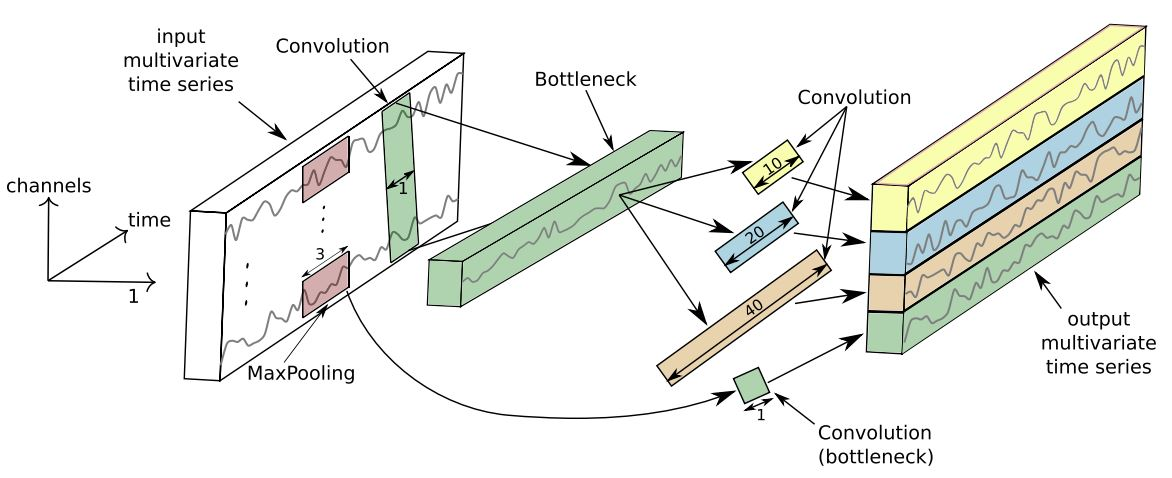
\includegraphics[scale = 0.5]{InceptionTime.JPG}
    \centering
    \caption{Inside Inception module for time series classification. For simplicity a bottleneck layer of size m = 1 is used \cite{fawaz2020inceptiontime}}
    \label{Img:InceptionTime}
\end{figure}

% Inception Ensemble
The final InceptionTime classifier is an ensemble of 5 InceptionTime networks.
InceptionTime networks accuracy scores showed high variances, a problem which have been discussed by \cite{scardapane2017randomness} and was found in ResNet networks as well \cite{fawaz2019deep}.
This happens due to the random initialization of the networks and due to the stochastic approach used for optimization.
InceptionTime classifier follows an ensembling technique for neural networks to handle TSC \cite{fawaz2019deep} in order to leverage the high variability;
adhering to the idea that combining multiple networks would yield better results than one classifier.
During the classification of an instance, InceptionTime combines the logistic output of the 5 networks and assigns an equal weight to each of them.
This can be denoted by the equation
\begin{equation}
    \hat{y}\textsubscript{i,c} = \frac{1}{n} \sum_{j = 1}^{n} \sigma\textsubscript{c} (x\textsubscript{i}, \theta\textsubscript{i}) | \forall\textsubscript{c} \epsilon [1,C]
\end{equation}
Where $\hat{y}\textsubscript{i,c}$ is the class probability for instance $x\textsubscript{i}$ as belonging to the class c,
which is the averaged logistic output $\sigma\textsubscript{c}$ over the randomly initialized models n.